\chapter{ Controlling the simulation }


\section{ General parameterisation }

 The general parameterisation of the computation is controlled using the steering file.


\subsection{ Computation title}

The computation case title is specified by the keyword \textit{TITLE}


\subsection{ Computation time}

The time data are prescribed using the two keywords \textit{TIME step} (real) and \textit{NUMBER OF TIME INCREMENTS }(integer). The
former sets the elapsed time, in seconds, between two consecutive computation instants (but not necessarily two outputs in the results
file). The number of time steps is for setting the overall computation time (which is obviously equal to the time increment value
multiplied by the number of time steps).

An additional keyword also refers to time. This is the \textit{DATE OF COMPUTATION BEGINNING}, which is used to identify the time in
relation to the date/times written in the \textit{WINDS FILE} (refer to \ref{se:desformat}, WAM-typed format). The convention adopted
for writing the \textit{DATE OF COMPUTATION BEGINNING} is yyyymmddhhmm. For instance, 190311051110 corresponds to November 5th, 1903, at
11.10 AM.

Note that when a computation is resumed, the initial time of the new computation corresponds to the last time increment in the previous
computation (i.e. the computation is not resumed at time zero).


\subsection{ Spectral discretisation}

 The spectral discretisation is defined by the following 5 keywords:  
\begin{itemize} 
\item  \textit{NUMBER OF DIRECTIONS}, \item     \textit{NUMBER OF FREQUENCIES}, \item    \textit{MINIMUM FREQUENCY}, \item
  \textit{FREQUENTIAL RATIO}, \item    \textit{SPECTRUM TAIL FACTOR}.
\end{itemize}
It should be reminded that the directions are evenly distributed from 0 to 360 degrees. Two conventions can be chosen by the user for
expressing the wave propagation by means of the keyword \textit{TRIGONOMETRICAL CONVENTION }(logical). The trigonometrical convention
locates the wave propagation from the positive X axis and the direction of rotation is in a counterclockwise direction. The default
convention is the nautical convention (\textit{TRIGONOMETRICAL CONVENTION} = NO) that locates the propagation direction in relation
to the true "North", i.e. the Y axis. The selected direction of rotation is a clockwise direction. The direction will then correspond
to the "heading" in the sense of the navigational maps, i.e. the direction the waves are propagating towards.

 The frequencies are distributed geometrically in accordance with the following relation:
\[f_{k} =f_{0} \; r^{k-1} \quad (k=1,NF)\]
where $f_{0} $ is the \textit{MINIMUM FREQUENCY }  r is the \textit{FREQUENTIAL RATIO}   NF is the \textit{NUMBER OF FREQUENCIES}

We can choose how to treat the high frequencies. If we want to impose the frequencies higher than the frequency cut off to decay
with a law of the type $f^{-n}$, then we set the \textit{OPTION FOR DIAGNOSTIC TAIL} to 1, and the \textit{SPECTRUM TAIL FACTOR }
corresponds to the value of n. The frequency cut off is the max of 4 Pierson-Moskowitz frequency and 2.5 mean frequency. 
The Pierson-Moskowitz frequency is defined as $\frac{g}{2\pi 28 u^*}$ where $ u^*$ is the friction wind velocity.  


\subsection{ Release}

When generating the executable, the release number of libraries being used for editing the links is indirectly provided by the
keyword \textit{\tomawac RELEASE NUMBER}. By default, \tomawac release 7.1 utilises the 7.1 releases of the TELEMAC system libraries.


\subsection{ Environment}

 When a vector computer is used, the CPU vector length used in the forced vectorisation technique can be specified by means of the keyword \textit{VECTOR LENGTH}. The default value is 1 and is appropriate for scalar machines such as the present workstations. If a value of 1 is used on a vector machine, then the advantage of the vectorisation loops (although they are few in \tomawac) is lost.


\section{ Computation options}


\subsection{ Co-ordinate system}

 Cartesian co-ordinates (expressed in meters) are used by default. For domains of a large extent, working in spherical co-ordinates may become necessary. The value of the logical keyword \textit{SPHERICAL COORDINATES} should then be set to "TRUE". The co-ordinates are then expressed in degrees.


\subsection{ Finite depth }

 In nearshore areas, wave conditions will be influenced by the water depth and therefore the bottom effect can no longer be ignored. This is the default case in \tomawac: the keyword \textit{INFINITE DEPTH }is set to ``FALSE''. In situations where depths effects are to be explicitly ignored the keyword \textit{INFINITE DEPTH} should be set to "TRUE".


\subsection{ Taking a stationary current into account}
\label{se:current}
A stationary current can be taken into account in the \tomawac. The relevant logical keyword is \textit{CONSIDERATION OF A STATIONARY
  CURRENT. }The current affects mainly the convection step.

 The current can be specified in various ways:

 When the current is either constant over the domain or can be described analytically, the ANACOS.f subroutine can be included in the
 FORTRAN file and modified accordingly. In this subroutine the UC and VC are NPOIN2-sized (number of points in the horizontal mesh)
 vectors and correspond to the components along the X and Y axes of the current, respectively. This is how the current is specified
 when the keyword \textit{FORMATTED CURRENTS FILE} or \textit{BINARY CURRENTS FILE }is not specified, whereas the keyword
 \textit{CONSIDERATION OF A STATIONARY CURRENT} is "TRUE".

 \tomawac can also take into account a current provided in a binary or formatted file. The keyword \textit{BINARY CURRENTS FILE} or
 \textit{FORMATTED CURRENTS FILE} should then be given a value (the name of the file). Three different formats are available to read
 this data. The value corresponds to the keyword \textit{CURRENTS FILE FORMAT} (see \ref{se:currentfile}). When the currents file is
 taken from TELEMAC-2D, then an additional keyword should be specified, namely the \textit{TIME INCREMENT NUMBER IN TELEMAC FILE.}
 This locates the desired record.

 If the predefined formats cannot be used, the USER\_CURRENT.f subroutine can be included in the FORTRAN and modified accordingly,
 specifying the format 4 for the INDIC FORTRAN variable in the CAS file. The current data are read from the file and are interpolated
 onto the nodes of the computation mesh.


\subsection{ Taking a wind into account}
\label{se:wind}
Consideration of a wind is specified by the logical keyword \textit{CONSIDERATION OF A WIND}. The wind may be either stationary or
variable in time and is specified by means of the logical keyword \textit{STATIONARY WIND}.

To Specify a constant wind in space, one can use keyword \textit{WIND VELOCITY ALONG X} and \textit{WIND VELOCITY ALONG Y}

When the wind can be described analytically, the user subroutine USER\_ANAVEN.f can be used. The wind is fully specified when the
keywords \textit{FORMATTED WINDS FILE} and \textit{BINARY WINDS FILE} do not have any value, whereas the keyword \textit{CONSIDERATION
  OF A WIND }is "TRUE".

\tomawac can also take into account a wind given in a binary or formatted file. In this case a value (the name of the file) should be
assigned to the keyword \textit{FORMATTED WINDS FILE }or \textit{BINARY WINDS FILE}. The available formats for reading out these data
correspond to the keyword \textit{WINDS FILE FORMAT} (see in section \ref{se:windfile} and \ref{se:desformat}).

When these predefined formats cannot be used, the subroutine USER\_WIND.f can be included in the FORTRAN file and modified accordingly,
specifying the format 4 for the INDIV FORTRAN variable. On completion of reading the winds file, the wind components are used as such
if provided on the computational mesh, or interpolated over that mesh in provided on a different grid.

NOTE: an interpolation between two different meshes of equivalent sizes is usually computationally very expensive. Although possible,
it is highly inadvisable, particularly as regards to the wind, since this is a time-varying data item. In such cases a
pre-interpolation over the computation mesh, e.g using STBTEL is recommended, followed by the reading of the wind data in format 3.
Alternatively this pre-interpolation can be performed by means of the FASP subroutine from the utils library.


\subsection{ Recovering a TELEMAC data item}
\label{se:telemacdata}
Recovering a 2D result data item from a TELEMAC-2D hydrodynamic computation might be of interest, e.g. the value of wind-driven
surge at every point. To avoid an increase in the number of files the \textit{BINARY CURRENTS FILE} is used to specify this input file.
The keyword \textit{CURRENTS FILE FORMAT} should then be set to 3. This option is further specified using the logical keyword
\textit{RECOVERY OF TELEMAC DATA ITEM}. The data item is located within the file through the \textit{TIME INCREMENT NUMBER IN TELEMAC
  FILE}.

NOTE: a TELEMAC data item and the components of a current can both be read simultaneously provided that they occur in the same file
at the same record.



\subsection{ Taking the tide into account}
\label{se:tide}
Tide-induced effects, i.e. unsteady/non-stationary water levels and currents can be taken in to account. The relevant logic keyword
is \textit{CONSIDERATION OF TIDE}.

In order to take tide into account, a current and a tide water depth that is referenced in relation to the "INITIAL STILL WATER LEVEL"
must be specified. These data can be initialized in various ways:

Should the tide be easy to describe analytically, the USER\_ANAMAR.f subroutine, can be included in the FORTRAN file and modified
accordingly. In the subroutine the terms UC and VC, ZM and DZHDT are NPOIN2-sized (number of points in the horizontal mesh) vectors
and correspond to the current components along the X and Y axes, the tidal water level in relation to the "INITIAL STILL WATER LEVEL"
and the water depth variation in time, respectively. An analytical expression must be assigned to all of these vectors.

\tomawac can also take into account a current that is given in a binary or formatted file. A value (the name of the currents file)
should be assigned to the keyword \textit{BINARY CURRENTS FILE} or\textit{ FORMATTED CURRENTS FILE}. Two different formats are available
for reading these data. This format is specified using the keyword \textit{CURRENTS FILE FORMAT} (see \ref{se:currentfile}). When these
predefined formats cannot be used, the user subroutine USER\_CURRENT.f can be included in the FORTRAN file and modified accordingly. In
such cases the \textit{CURRENTS FILE FORMAT} (FORTRAN variable INDIC) must be set to 4 in the CAS file. Once the data of the currents
file are read, the current components are interpolated over the computation mesh.

The tidal water level can be also provided in a binary or formatted file. A value (the name of the water level file) should be
assigned to the keyword \textit{BINARY TIDAL WATER LEVEL FILE} or\textit{ FORMATTED TIDAL WATER LEVEL FILE}. Two different predefined
formats are available for reading this data. The format type is specified using the keyword \textit{TIDAL WATER LEVEL FILE FORMAT}
(refer to \ref{se:tidalfile}). If the user chooses the Serafin format (i.e. TELEMAC-2D format), then the \textit{RANK OF THE WATER
  LEVEL DATA IN THE TELEMAC FILE} must also be specified. When the predefined formats cannot be used, the user subroutine
USER\_TIDE.f file can be included in the FORTRAN file and modified accordingly. In such cases the \textit{TIDAL WATER LEVEL FILE FORMAT}
(the INDIM FORTRAN variable) must be set to 4 in the CAS file.

Both currents and tidal water levels will be updated upon each \textit{TIDE REFRESHING PERIOD}. This keyword corresponds to an integer
multiple of the propagation \textit{TIME STEP}, i.e. the currents and tidal levels cannot be specified at time steps less than the
model TIME STEPS\textit{.}


\subsection{ Waves-current interactions: direct coupling with Telemac (2D or 3D) flow simulation}

It is possible to directly couple a \tomawac and a \telemac{} simulation (either TELEMAC-2D or TELEMAC-3D) to represent the wave-current
interactions more precisely.

In \tomawac, when the keywords \textit{CONSIDERATION OF A TIDE} or \textit{CONSIDERATION OF A STATIONARY CURRENT} are used, the current
is imposed as an input data: in this case only the effect of the current on the waves is taken into account, but not the effect of the
waves on the current. The current imposed, therefore, is not affected by the waves and can differ from the real current interacting
with the waves.

By using a direct coupling TELEMAC-\tomawac it is possible to represent wave current interactions in both directions: TELEMAC transfers
to \tomawac the updated values of current velocities and water depths, while \tomawac solves the wave action density conservation
equation with reference to those current and water depth values and returns to \telemac the updated values of the wave driving forces
FX and FY acting on the current.

To directly couple a TELEMAC model with a \tomawac model, the following conditions must be satisfied:

\begin{itemize}

\item  the TELEMAC and \tomawac simulations must have the same simulation time length (given by the time step multiplied by the number
  of time steps)

\item  the time steps set for the two simulations must be equal or multiple of each other

\item  current and/or water level file cannot be used as input data for the \tomawac simulation

\item  the driving force along X and Y (\textit{FX}, \textit{FY}) must be set among the 2D output variables in the steering file
\end{itemize}

There are two kinds of coupling, in the first one the \telemac{} and \tomawac models must have the same horizontal mesh. Using tel2tom
you are allowed to have different meshes with interpolation of variables between the 2 meshes. In that case the weight of
interpolations must have been calculated before the simulation and must be recorded in the meshes. This can be done using the command
{\it run\_telfile.py tel2tom}. An example of use of this command is done in the notebook : {\it pretel/tel2tom.ipynb}

In case of direct coupling TELEMAC-\tomawac, TELEMAC is the main programme and calls the \tomawac subroutine WAC, which is the main
subroutine of \tomawac and solves the equation of generation and propagation of the directional wave spectrum.

The TELEMAC-\tomawac coupling is set via four keywords in the TELEMAC steering file:

\begin{itemize}
\item  \textit{COUPLING WITH}, to which the value '\tomawac' must be assigned for the first kind of coupling. If you want to use
  tel2tom and have different meshes for \tomawac and \telemac{} the value TOMAWAC2 must be assigned. 
\item  \textit{WAVE DRIVEN CURRENT} must be set to 1

\item  \textit{\tomawac STEERING FILE}, which specifies the name of the \tomawac steering file: its path must be specified with
  reference to the working directory of the TELEMAC steering file.

\item  \textit{COUPLING PERIOD FOR \tomawac} (variable \textit{PERCOU\_WAC),} which specifies how many TELEMAC time steps \tomawac
  is called:

\begin{itemize}
\item  The \tomawac time step must be less or equal TELEMAC simulation time step multiplied by PERCOU\_WAC.

\item  The ratio of the two time steps must be an integer.
\end{itemize}
\end{itemize}

Different examples are given in {\it gaia/littoral-t2d-tom} and {\it Coupling\_Wind}.

In the case of coupling with \telemac{3D}, you can also make the difference between a 2D coupling and a real 3D coupling.
To specify that you want a 3D coupling you have to add {\it T3D} after coupling with tomawac (see the documentation of \telemac{3D}).
Some examples of this 3D coupling are given in the test cases ({\it Rip} and {\it 3Dcoupling}).

All the file names specified in the \tomawac steering file (geometry file, boundary conditions file, Fortran file, 
\dots ) must be given as paths relative to the working directory of the TELEMAC steering file. Note that, when you
use direct coupling, you are not allowed to read a wind in \tomawac: wind must be transmitted by \telemac{2D} or \telemac{3D}

For more information concerning the modelling options in \telemac{}, please refer to the \telemac{} documentation.

\subsection{ Convection step}

For specific validation tests, for example, it may be interesting to drop the convection step and only consider the effect of the
source terms. To do this requires assigning the "FALSE" value to the keyword \textit{CONSIDERATION OF PROPAGATION}.


\subsection{ Taking diffraction into account}

 Diffraction can be included in \tomawac simulations only if the following conditions are fulfilled:
\begin{itemize}

\item The spatial mesh is defined in terms of Cartesian coordinates.

 \item Neither currents nor time-varying levels are taken into account.

 \item The simulation is run sequentially and not in parallel mode.
\end{itemize}

Four keywords can be used to parameterize the representation of diffraction in \tomawac:

\begin{itemize}
\item  \textit{DIFFRACTION}: its default value is zero, and corresponds to the case in which diffraction is not taken into account.
  If \textit{DIFFRACTION} is set to one, diffraction is considered and the Mild Slope Equation (MSE) approach is applied. If
  \textit{DIFFRACTION} is set to two, diffraction is considered and the Revised Mild Slope Equation (RMSE) approach is applied.

\item  \textit{STARTING TIME STEP FOR DIFFRACTION}: it indicates at which time step of the simulation diffraction is taken into account.
  Its default value is 1 (i.e. diffraction is solved from the first time step). When diffraction is considered in \tomawac simulations,
  the computing time is longer. To reduce it, it is recommended to set \textit{STARTING TIME STEP FOR DIFFRACTION} at a value
  corresponding approximately to the time step at which the same \tomawac model, without the consideration of diffraction, reaches a
  steady-state.

\item  \textit{VARIANCE THRESHOLD FOR DIFFRACTION}: it indicates the minimum spectral variance threshold considered when diffraction is
  taken into account. The default value is 1E-12.

\item  \textit{DIFFRACTION FILTER}: if TRUE, it indicates that the filtering of the local amplitudes of directional spectra is carried
  out when diffraction is considered.
\end{itemize}

The diffraction module implemented in \tomawac is able to capture the diffusion of the wave height behind diffracting structures, but
\textbf{it is not adapted to represent in detail the diffracted wave field}.

 The first version of the diffraction module implemented in \tomawac presents still several limits that must be overcome:

\begin{itemize}
\item  Unrealistic energy build-up and numerical noise are generated when diffraction is taken into account: at a constant Courant
  number, the smaller the mesh element size to wavelength ratio, the larger the numerical instability.

\item  The simulation results are very sensitive to the Courant number and to the ratio between the mesh element size and the
  wavelength associated to the peak period.

\item  In the case of a complex and rapidly varying bathymetry (e.g. a submerged shoal case), the model underestimates the effect of
  diffraction.
\end{itemize}

 For problems in which diffraction must be simulated precisely (e.g. harbor agitation), the use of phase-resolving model is recommended.

 The following recommendations can be made, in order to build and run a \tomawac model in which diffraction is taken into account:

\begin{itemize}
\item  A too fine mesh can lead to numerical noise and unsteadiness in the results, while with a mesh too coarse the diffraction
  effect is underestimated. The best compromise found so far for the parameterization of \tomawac is to set the ratio between the
  smallest mesh element size and the wavelength associated to the peak period $\Delta X/\Lambda$ within the interval 0.2-0.25 (i.e.
  approximately 4 to 5 mesh elements per wavelength)

\item  When setting the Courant number \textit{Cr}, a compromise must be found between the computing time required (large values of
  \textit{Cr} imply shorter computing times) and a low numerical noise in the solution (the lower \textit{Cr}, the lower the numerical
  noise). For values of  $\Delta X/\Lambda$ within the interval 0.2-0.25 a Courant number Cr not larger than 0.1 is recommended.

\item  A numerical smoothing filter can improve the simulation results, especially when using a mesh with a very high spatial resolution
  (small $\Delta X/\Lambda$, i.e. when numerical noise and energy build-up are generated during the simulation. The filter smoothens in
  the spatial domain the local amplitude of the directional spectrum.
\end{itemize}


\section{ Parameterising the source term integration step}


\subsection{ Introduction}

When it is required to take into account the source/sink terms, the logic keyword \textit{CONSIDERATION OF SOURCE TERMS }should be set
to "TRUE".

It has been shown that the source term integration may require a shorter time step than the time step that is used for convection. The
\textit{TIME STEP} in the steering file corresponds to the convection time step. The source term integration step is controlled using
the integer keyword \textit{NUMBER OF ITERATIONS FOR THE SOURCE TERMS.} This keyword is set to the number of source terms integration
time steps that will be conducted after each convection step (default value = 1). The effective time-step used for source term
integration is thus:

 \textit{(TIME STEP)/(NUMBER OF ITERATIONS FOR THE SOURCE TERMS).}

 Depending on the source/sink terms, two different schemes are used for time integration:

\begin{itemize}
\item  For the source/sink terms which are dominant in large and medium water depths (namely wind input, white-capping dissipation,
  nonlinear quadruplet interactions and bottom friction) a scheme with variable implicitation level is used (see section
  \ref{se:sourclarge}
).

\item  For the source/sink terms which are dominant in shallow water depths (namely depth-induced breaking and, nonlinear triad
  interactions) an explicit scheme is used, possibly with sub-steps to cover one source term time-step (see section
  \ref{se:sourcshallow}).
\end{itemize}


\subsection{ Source/sink terms in large and medium water depth}
\label{se:sourclarge}

\paragraph{ Wind input}

 In \tomawac three wind generation models and a linear wave growth model are available (see section 4.2.3.2 for details).

 If the keyword \textit{WIND GENERATION} is set to 0, no wind input will be taken into account. If, on the other hand, a strictly
 positive value is chosen, the corresponding wind input formulation will be taken into account.

 \underline{ The Janssen formulation} is activated using the value 1 for the WIND GENERATION keyword. Janssen's formulation requires
 several additional data, specified by the following keywords:
 
- \textit{AIR DENSITY},

- \textit{WATER DENSITY},  

- \textit{WIND GENERATION COEFFICIENT}, 

- \textit{VON KARMAN CONSTANT}, 

- \textit{CHARNOCK CONSTANT},   

- \textit{SHIFT GROWING CURVE DUE TO WIN,} 

- \textit{WIND DRAG COEFFICIENT},  

- \textit{WIND MEASUREMENT LEVEL}.  

  \textit{}

As a general rule, the default values for these keywords shall not be modified.

\underline{ The Snyder formulation} is activated setting to 2 the value for the WIND GENERATION keyword and uses two parameters,
specified by the following keywords:   

- \textit{AIR DENSITY},   

- \textit{WATER DENSITY},

   \textit{}

   \underline{ The Yan formulation} is activated setting to 3 the value for the WIND GENERATION keyword and uses four parameters,
   specified by the following keywords:   

- \textit{YAN GENERATION COEFFICIENT D}  

- \textit{YAN GENERATION COEFFICIENT E} 

- \textit{YAN GENERATION COEFFICIENT F} 

- \textit{YAN GENERATION COEFFICIENT H}

  \textit{}

As a general rule, the default values for these keywords shall not be modified.

\underline{  The linear wave growth model}, based on the Cavaleri \& Malanotte-Rizzoli formulation, is activated setting to 1 the
keyword \textit{LINEAR WAVE GROWTH}. This formulation does not require any additional data to be specified by the user.


\paragraph{ White capping dissipation}

 In \tomawac two whitecapping dissipation models are available (see section 4.2.3.2 for details).

 If the integer keyword \textit{WHITE CAPPING DISSIPATIO} is set to 0, this source term will be ignored. If a strictly positive value
 is selected, the corresponding formulation will be taken into account.

 \underline{  The Komen's formulation} corresponds to the value 1 of the \textit{WHITE CAPPING DISSIPATION} keyword. This formulation requires two complementary data, specified by the following keywords:   

- \textit{WHITE CAPPING DISSIPATION COEFFICIENT}   

- \textit{WHITE CAPPING WEIGHTING COEFFICIENT}.

  \textit{}

 As a general rule, the default values for these keywords shall not be modified.

 \underline{  The Westhuysen formulation} corresponds to the value 2 of the \textit{WHITE CAPPING DISSIPATION} keyword. This formulation requires four complementary data, specified by the following keywords:  

-  \textit{WESTHUYSEN DISSIPATION COEFFICIENT}

-  \textit{SATURATION THRESHOLD FOR THE DISSIPATION}

-  \textit{WESTHUYSEN DISSIPATION MODEL WHITE CAPPING DISSIPATION}

-  \textit{WESTHUYSEN DISSIPATION MODEL WEIGHTING COEFFICIENT}

  \textit{}

As a general rule, the default values for these keywords shall not be modified.

\paragraph{ Bottom friction dissipation}

If the integer keyword \textit{BOTTOM FRICTION DISSIPATION} is set to 0, this source term will be ignored. If a strictly positive
value is chosen, the corresponding formulation will be taken into account. This source term is only taken account if the keyword
\textit{INFINITE DEPTH} is set to "FALSE".

The only formulation implemented is from Hasselmann (see section 4.2.3.4 for details) This formulation is specified by setting the
\textit{BOTTOM FRICTION DISSIPATION} keyword to 1. This formulation requires the specification of the keyword:

  - \textit{BOTTOM FRICTION COEFFICIENT}.

 As a general rule, the default value for this keyword shall not be modified.


\paragraph{ Non-linear transfers between quadruplets}

Three non-linear quadruplet interactions models are available in \tomawac (see in section 4.2.3.6). The non-linear quadruplet
interactions are activated through the keyword \textit{NON-LINEAR TRANSFERS BETWEEN FREQUENCIES} in the steering file; the keyword
can take four values.

If the integer keyword \textit{NON-LINEAR TRANSFERS BETWEEN FREQUENCIES} is set to 0, this source term will not be taken into account.
If a strictly positive value is chosen, the corresponding formulation will be taken into account.

\underline{  The DIA method} (formulation from \cite{Hasselmann1985_1}) corresponds to the value 1 for the \textit{NON-LINEAR TRANSFERS
  BETWEEN FREQUENCIES} keyword. This formulation does not require any additional data to be specified by the user.

\underline{The MDIA method }(formulation from \cite{Tolman2004}) corresponds to the value 2 for the \textit{NON-LINEAR TRANSFERS
  BETWEEN FREQUENCIES} keyword. This formulation does not require any additional data to be specified by the user.

\underline{The qausi-excat GQM method} (formulation based on \cite{Lavrenov2001}) corresponds to the value 3 for the \textit{NON-LINEAR
  TRANSFERS BETWEEN FREQUENCIES} keyword. This formulation requires the specification of six keywords:

- \textit{SETTING FOR INTEGRATION ON OMEGA1}

- \textit{SETTING FOR INTEGRATION ON THETA1}

- \textit{SETTING FOR INTEGRATION ON OMEGA2}

- \textit{THRESHOLD0 FOR CONFIGURATIONS ELIMINATION}

- \textit{THRESHOLD1 FOR CONFIGURATIONS ELIMINATION}

- \textit{THRESHOLD2 FOR CONFIGURATIONS ELIMINATION}


\subsection{ Source/sink terms in shallow water depth}
\label{se:sourcshallow}

\paragraph{ Time integration scheme and time step}

 As mentioned above, the depth-induced breaking and nonlinear triad interaction terms are time-integrated with an explicit scheme.

 As found practically, contributions from these source terms can be overestimated if the selected time step for source term integration
 is too long. In order to avoid this, \tomawac can perform a number of time sub-steps which are specific to these source terms through
 the keyword \textit{NUMBER OF BREAKING TIME STEPS}.

 These time sub-steps are arranged in a geometrical progression, i.e. they are defined in the following way:

dt${}_{i+1 }$= q dt${}_{i}$

 where the geometrical ratio q is specified through the keyword: \textit{COEFFICIENT OF THE TIME SUB-INCREMENTS FOR BREAKING}

 In order to limit this number of time-steps, \tomawac first clips the wave height by setting a maximum H${}_{m0}$/D ratio (D is the
 water depth) to 1. This ratio can be modified by means of the keyword \textit{MAXIMUM VALUE OF THE RATIO HM0 TO D}. However, this is
 generally not advisable.


\paragraph{ Wave breaking dissipation}

If the integer keyword \textit{DEPTH-INDUCED BREAKING DISSIPATION} is taken as 0, this source term will be ignored. If a strictly
positive value is chosen, the corresponding formulation will be taken into account.

 Four formulations have been implemented (see section 4.2.3.5 for details):

 \textbf{\underbar{1: Battjes and Janssen's model (1978)}}

 This formulation requires additional data to be provided, specified by the following keywords:

 - \textit{DEPTH-INDUCED BREAKING 1 (BJ) COEFFICIENT ALPHA}

 - \textit{DEPTH-INDUCED BREAKING 1 (BJ) COEFFICIENT GAMMA1}

 - \textit{DEPTH-INDUCED BREAKING 1 (BJ) COEFFICIENT GAMMA2}

 - \textit{DEPTH-INDUCED BREAKING 1 (BJ)CHARACTERISTIC FREQUENCY }

 - \textit{DEPTH-INDUCED BREAKING 1 (BJ)QB COMPUTATION METHOD}

 \textit{}

 \textbf{\underbar{2: Thornton and Guza's model (1983)}}

 This formulation requires additional data to be provided, specified by the following keywords:

 - \textit{DEPTH-INDUCED BREAKING 2 (TG) COEFFICIENT B}

 - \textit{DEPTH-INDUCED BREAKING 2 (TG) COEFFICIENT GAMMA}

 - \textit{DEPTH-INDUCED BREAKING 2 (TG) WEIGHTING FUNCTION}

 \textit{- DEPTH-INDUCED BREAKING 2 (TG) CHARACTERISTIC FREQUENCY}

 \textbf{}

 \textbf{\underbar{3: Roelvink's model (1993)}}

 This formulation requires additional data to be provided, specified by the following keywords:

 - \textit{DEPTH-INDUCED BREAKING 3 (RO) COEFFICIENT ALPHA}

 - \textit{DEPTH-INDUCED BREAKING 3 (RO) COEFFICIENT GAMMA}

 - \textit{DEPTH-INDUCED BREAKING 3 (RO) COEFFICIENT GAMMA2}

 \textit{- DEPTH-INDUCED BREAKING 3 (RO) WAVE HEIGHT DISTRIBUTION}

 \textit{- DEPTH-INDUCED BREAKING 3 (RO)EXPONENT WEIGHTING FUNCTION}

 \textit{- DEPTH-INDUCED BREAKING 3 (RO)CHARACTERISTIC FREQUENCY}

 \textbf{}

 \textbf{\underbar{4: Izumiya and Horikawa's model (1984)}}

 This formulation requires additional data to be provided, specified by the following keywords:

 - \textit{DEPTH-INDUCED BREAKING 4 (IH) COEFFICIENT BETA0}

 - \textit{DEPTH-INDUCED BREAKING 4 (IH) COEFFICIENT M2STAR}

 - \textit{DEPTH-INDUCED BREAKING 4 (IH) CHARACTERISTIC FREQUENCY}

\paragraph{ Triad interactions}

If the integer keyword \textit{TRIAD INTERACTIONS} is set to 0, this source term will be ignored. If a strictly positive value is
specified, the corresponding formulation will be taken into account.

 Two formulations (see section 4.2.3.7) have been implemented.

 \textbf{\underbar{1: LTA model}}

 This formulation requires additional associated data to be specified using the following keywords:

 - \textit{TRIADS 1 (LTA) COEFFICIENT ALPHA }

 \textit{- TRIADS 1 (LTA) COEFFICIENT RFMLTA }

 \textbf{}

 \textbf{\underbar{2: SPB model}}

 This formulation requires additional associated data to be specified using the following keywords:

 - \textit{TRIADS 2 (SPB) COEFFICIENT KTRIADS 2 (SPB) COEFFICIENT K}

 \textit{- TRIADS 2 (SPB) LOWER DIRECTIONAL BOUNDARY}

 \textit{- TRIADS 2 (SPB) UPPER DIRECTIONAL BOUNDARY}

 ATTENTION: the SPB model is very time-consuming; compared to the LTA model formulation, it requires a computational time approximately 700 times higher.


\paragraph{ Wave blocking }

 If the integer keyword \textit{DISSIPATION BY STRONG CURRENT} is set to 0, this source term will be ignored. If a strictly positive (1 or 2) is specified, the corresponding formulation will be taken into account.

 \textbf{\underbar{1: Upper limit for spectrum}} : We locally use a Phillips's constant of 0.0081 to build a limit spectrum. This does not change the value of Phillip's constant in the entire code.  

 \textbf{\underbar{2: Westhuysen formulation :}}

 This Westhuysen formulation requires 2 parameters.

 - \textit{DISSIPATION COEFFICIENT FOR STRONG CURRENT}

 - \textit{SATURATION THRESHOLD FOR THE DISSIPATION}

 Caution : the second coefficient is the one used in the white capping formulation of Westhuysen \cite{Westhuys2008}.


\paragraph{ Vegetation dissipation}

If logical keyword \textit{VEGETATION TAKEN INTO ACCOUNT} is set to true, then vegetation is taken into account. As the
parameters are case-specific, the parameters should be modified through the fortran user subroutine \textit{QVEG. }In this
subroutine the user will give the value $\tilde{C}_{D} $, the vegetation drag coefficient, \textit{b${}_{v}$} [m] the stem diameter
of cylinder (plant), \textit{N${}_{v}$} [-] the number of plants per square meter and $\alpha $the ratio between vegetation height
and water depth.

\paragraph{ Vegetation dissipation}

If logical keyword \textit{VEGETATION TAKEN INTO ACCOUNT} is set to true, then vegetation is taken into account. As the parameters
are case-specific, the parameters should be modified through the fortran user subroutine \textit{QVEG. }In this subroutine the user
will give the value $\tilde{C}_{D} $, the vegetation drag coefficient, \textit{b${}_{v}$} [m] the stem diameter of cylinder (plant),
\textit{N${}_{v}$} [-] the number of plants per square meter and $\alpha $the ratio between vegetation height and water depth.

\paragraph{Porous Media}

If logical keyword \textit{POROUS MEDIA} is set to true, then vegetation is taken into account. As the parameters are case-specific,
the parameters should be modified through the fortran user subroutine \textit{QPOROS}. In this subroutine the user will give the
value of porosity rate, (\textit{TAU}), the damping mass coefficient (\textit{CA}),  the linearised friction coefficient
(\textit{coeff}) and the thickness rate of the porous medium (\textit{alpha}).

 \section{ Prescribing the initial conditions}
\label{se:initcond}
 Initial conditions can be prescribed using the integer keyword \textit{TYPE OF INITIAL DIRECTIONAL SPECTRUM}.

 Table \ref{tab:Jonswap} shows all the available options in \tomawac for computing the frequential and directional distribution of
 wave action. It should be remembered that the variance density directional spectrum is computed as the product:
\[F(f,\theta )=E(f).D(\theta )\]
where $E(f)$ here denotes the variance density spectrum and $D\left(\theta \right)$ denotes the angular distribution function.

 It is reminded that the parameterised JONSWAP spectrum is defined as:
 \[E(f)=\alpha _{phil} g^{2} (2\pi )^{-4} f^{-5} \exp \left[-\frac{5}{4} \left(\frac{f_{p}^{} }{f^{} } \right)^{4} \right]
 \gamma ^{\exp \left[-\frac{\left(f-f_{p} \right)^{2} }{2\sigma ^{2} f_{p}^{2} } \right]} \]
 where:  $\sigma =\sigma_{a} =0.07$ for  $f< f_{p}$  and  $\sigma =\sigma_{b} =0.09$ for  $f> f_{p}$. Here, $\alpha_{phil}$  is
 the Phillips constant that can be specified in the parameter file (keyword INITIAL PHILLIPS CONSTANT).

 If one wants to parametrize the formula with $H_{m0}$ (case 5 with wind and case 6), one writes
 \[E(f)=\alpha _{phil} H_{mo}^{2} \frac{f_{p}^{4} }{f^{5} } \exp \left[-\frac{5}{4} \left(\frac{f_{p}^{} }{f^{} } \right)^{4} \right]
 \gamma ^{\exp \left[-\frac{\left(f-f_{p} \right)^{2} }{2\sigma ^{2} f_{p}^{2} } \right]} \]
With $\dsp \alpha _{phil} =\frac{0.0624}{0.23+0.0336\gamma -\frac{0.185}{1.9+\gamma } } $ as done in Tomawac.

 In case 7, the TMA spectrum is a depth-corrected JONSWAP-type spectrum.

 A parameterised spectrum with two directional peaks can also be generated. In such case, both main propagation directions
 ($\theta _{1} $ and $\theta _{2} $) as well as the weighting factor ($\lambda $) between the two power peaks:
 \[D(\theta )=\frac{\lambda }{\Delta _{1} } \tilde{D}(\theta -\theta _{1} )+\frac{1-\lambda }{\Delta _{2} } \tilde{D}(\theta -
 \theta _{2} )\]
must be specified.

$\Delta_{1}$ and $\Delta_{2,}$ in the equation above, are automatically computed by \tomawac in order to normalize the angular
distribution function.

Three angular distribution functions may be chosen using the keyword \textit{INITIAL ANGULAR DISTRIBUTION FUNCTION}, which
correspond to the following options:

 1: model in $\cos ^{2s} (\theta -\theta _{0} )$~; $\theta \in \left[\theta _{0} -\pi /2\; ;\; \theta _{0} +\pi /2\right]$

 2: model in $\exp \left(-0.5\left(\left(\theta -\theta _{0} \right)/s\right)^{2} \right)$~; $\theta \in \left[\theta _{0} -
   \pi /2\; ;\; \theta _{0} +\pi /2\right]$

 3: model in $\cos ^{2s} \left(\left(\theta -\theta _{0} \right)/2\right)$ ; $\theta \in \left[\theta _{0} -\pi \; ;\; \theta _{0}
   +\pi \right]$ Mitsuyasu \cite{Mitsuyasu1975}

 4: same than 3 but with
 $ s=\left\{ \barr{l} s_{max} \left(\frac{f}{f_p} \right)^5 : f\le f_p \\
 s_{max} \left(\frac{f}{f_p} \right)^{-2.5} : f > f_p \earr\right. $ as proposed by Goda et al. \cite{Goda1975}. 
 
 with $\theta_{0}$ being the main sea-state propagation direction and \textit{s} being the directional spread. According to
 \cite{Goda1975}, $s_{max}$ should be 10, 25 and 75 for wind waves, swell with short decay distance, and swell with long decay
 distance.

 The forementioned constants can be specified using the following of keywords:

 $H_{m0}$: \textit{INITIAL SIGNIFICANT WAVE HEIGHT},

 $f_p$:  \textit{INITIAL PEAK FREQUENCY},

 $\gamma$:  \textit{INITIAL PEAK FACTOR},

 $\sigma_a$:  \textit{INITIAL VALUE OF SIGMA-A FOR SPECTRUM},

 $\sigma_b$:  \textit{INITIAL VALUE OF SIGMA-B FOR SPECTRUM},

 $\alpha_{phil}$:  \textit{INITIAL PHILLIPS CONSTANT},

 $Fetch$:  \textit{INITIAL MEAN FETCH VALUE},

 $f_{pmax}$:  \textit{INITIAL MAXIMUM PEAK FREQUENCY},

 $\theta_1$:  \textit{INITIAL MAIN DIRECTION 1},

 $s1$:  \textit{INITIAL DIRECTIONAL SPREAD 1},

 $\theta_2$:  \textit{INITIAL MAIN DIRECTION 2},

 $s2$:  \textit{INITIAL DIRECTIONAL SPREAD 2},

 $\lambda$:  \textit{INITIAL WEIGHTING FACTOR FOR ADF},


 The keyword \textit{SPECTRUM ENERGY THRESHOLD} is used whatever option is chosen. It is only useful for comparisons with
 the WAM model.

 Specific initial conditions can be prescribed directly for the directional spectrum of wave action using the condiw.f
 subroutine which can be called from the speini.f subroutine.

\begin{table}
%\begin{tabular}{|p{0.45in}|p{0.55in}|p{2.2in}|p{0.8in}|} \hline
\begin{tabular}{|c|c|p{2.2in}|p{1.8in}|} \hline
Key- &  &  &  \\ 
word  &  & Spectrum & Constants  being used \\ 
 value &  & &  \\ \hline
0 &  & Zero spectrum & none \\ \hline
1 & Wind$\ne 0$ & - Frequencies: Jonswap according to wind  \newline - Directions: unimodal about the wind $(\theta_1 = \theta_w)$&
$f_{pmax}$, $ \gamma $, $ \sigma_a$, $ \sigma_b$, $Fetch$, $ s_1 $  \\ \hline
 & Wind=0 & Zero spectrum & none \\ \hline
2 & Wind$\ne 0$ & - Frequencies: Jonswap according to wind \newline - Directions: unimodal about the wind $(\theta_1 = \theta_w)$ &
$f_{pmax}$, $ \gamma $, $ \sigma_a$, $ \sigma_b$, $Fetch$, $ s_1 $ \\ \hline
& Wind=0 & - Frequencies: parameterised Jonswap $(\alpha , f_p)$ \newline - Directions: parameterised unimodal
(same spectrum at every point) & $\alpha_{phil}$, $ f_p$, $ \gamma $, $ \sigma_a$, $ \sigma_b$, $ s1$, $ \theta_1$ \\ \hline
3 & Wind$\ne0$ & - Frequencies: parameterised Jonswap $(\alpha)$ \newline - Directions: unimodal about the wind $(\theta_1 = \theta_w)$ &
$\alpha_{phil}$, $ f_p$, $ \gamma $, $ \sigma_a$, $ \sigma_b$, $ s1$ \\ \hline
 & Wind=0 & Zero spectrum & none \\ \hline
4 &  & - Frequencies: parameterised Jonswap $(\alpha , f_p)$  \newline  - Directions: parameterised angular distribution function.
Same spectrum at every point& $\alpha_{phil}$, $ f_p$, $ \gamma $, $ \sigma_a$, $ \sigma_b$, $ s1$, $ \theta_1$, $ s2$, $ \theta_2$,
$ \lambda$ \\ \hline
% & Wind=0 & - Directions: parameterised angular distribution function. Same spectrum at every point & $\alpha_{phil}$, $ f_p$,
$ \gamma $, $ \sigma_a$, $ \sigma_b$, $s1$, $ \theta_1$, $ s2$, $ \theta_2$, $ \lambda$ \\ \hline
5 & Wind$\ne 0$ & - Frequencies: parameterised Jonswap $(H_{m0})$ \newline - Directions: unimodal about the wind  $(\theta_1 = \theta_w)$
& $H_{m0}$, $ f_p$, $ \gamma $, $ \sigma_a$, $ \sigma_b$, s1 \\ \hline
 & Wind=0 & Zero spectrum & none \\ \hline
6 &  & - Frequencies: parameterised Jonswap  $(H_{m0}, f_p)$  \newline - Directions: parameterised angular distribution function.
Same spectrum at every point& $H_{m0}$, $ f_p$, $ \gamma $, $ \sigma_a$, $ \sigma_b$, $s1$, $ \theta_1$, $ s2$, $ \theta_2$, $ \lambda$ \\
\hline
% & Wind=0 & - Directions: parameterised angular distribution function. Same spectrum at every point &  \\ \hline
7 &  & - Frequencies: parameterised TMA $(H_{m0}, f_p)$ \newline - Directions: parameterised angular distribution function. Same
spectrum at every point & $H_{m0}$, $ f_p$, $ \gamma $, $ \sigma_a$, $ \sigma_b$, $s1$, $ \theta_1$, $ s2$, $ \theta_2$, $ \lambda$ \\
\hline
% & Wind=0 & - Directions: parameterised angular distribution function. Same spectrum at every point &  \\ \hline
\end{tabular}
\caption{\label{tab:Jonswap}Summary table of the spectrum types as proposed in \tomawac}
\end{table}



\section{  Prescribing the boundary conditions}

The boundary conditions are prescribed over the \underbar{relative} spectrum of wave action, i.e. expressed in co-ordinate system
that moves with the current.

 There are three kinds of boundary conditions are available in \tomawac.

 The first one corresponds to a free boundary i.e. a boundary that fully absorbs the wave energy. It may be a liquid boundary: it
 is then assumed that the waves propagate beyond the domain and nothing else enters it. It may be a solid boundary: it is
 then assumed that the shore fully absorbs the wave energy. The colour of this condition will begin by 2, and will be 2 2 2 2
 to be consistent with telemac.
 
 The second one corresponds to a boundary with a prescribed value. In this case the wave action spectrum is then strictly imposed at
 each point along that boundary. This boundary condition allows wave energy to enter the computational domain. The imposed
 spectro-angular spectrum can be given by analytical function such as a jonswap (see \ref{tab:Jonswap}) or imposed by an imposed spectra file (see
 \label{se:ImpSpeCoorFiles}). The colour of this condition will start with 5 and will be 5 4 4 4 to be consistent with telemac.

 The third one corresponds to a reflective boundary. As there are no natural expression to have a reflective condition with the
 equations governing waves propagation in Tomawac, this condition is more a source dependending on the incoming wave. At each point of
 this boundary for each frequency and each direction of the incoming wave, we construct a source with the direction transmitted
 following the law of Snell Descartes(see \ref{fig:reflection}) and projected on the discretised directions.

\begin{figure}[H]%
\begin{center}
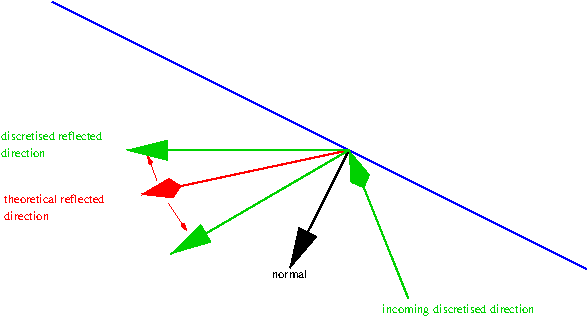
\includegraphics[width=0.9\textwidth]{graphics/reflection}
\caption{scheme of reflection in \tomawac}
\label{fig:reflection}
\end{center}
\end{figure}

To have reflection the user must set the keyword \textit{REFLECTION} to \textit{YES} (default is \textit{NO})
The user can also specify a coefficient of reflection, by the keyword \textit{REFLECTION COEFFICIENT} (the default is 1).
The colour of reflection condition must start by 8 and will be 8 4 4 4 to be consistent with telemac.

 The boundary conditions are specified using the boundary conditions (CONLIM) file, the steering (CAS) file and the LIMWAC.f.


 \subsection{ The boundary conditions file}

 \subsubsection{The Serafin boundary condition file}
\label{se:BCfile}
The boundary condition (CONLIM) file is normally supplied by STBTEL (or other TELEMAC mesh generators), but it can also be generated
by means of a text editor. Each line in this file is assigned to one point of the boundary and listed in sequential order in terms of
the boundary node numbers. The numbering of the boundary points first delineates the domain contour in a counterclockwise direction,
then the islands in the
clockwise direction. The total number of edge points is noted as NPTFR.

 13 values are given for each point. Only data in colums 1, 12 and 13 are used by \tomawac:

\begin{itemize}
\item The 13th data column (integer variable IPTFR) corresponds to the boundary point number ranked in terms of the boundary point
  numbering.
\item The 12th data column (integer variable IPOIN) corresponds to the global number of the point in the 2D mesh.
\item Lastly, the 1st data column (integer variable LIFBOR) corresponds to the kind of boundary condition. Consistent with TELEMAC-2D,
  its  value is 2 in the case of a free boundary and 5 in the case of a boundary with a prescribed value.
\end{itemize}

\subsubsection{The Med boundary condition file}
In that case each line of the file gives the colour of a group of segment. To be consistent with \telemac2d 4 colours has to be given
but only the first one is taken into account by tomawac. Each points belonging to the segments of the group will then have the colour
designed. 


\subsection{ Prescribing the boundary conditions in the CAS file}

 Boundary conditions prescribed using the CAS file will necessarily be homogeneous all along the domain entry boundaries.

 The boundary conditions can be prescribed by means of the integer keyword \textit{TYPE OF BOUNDARY DIRECTIONAL SPECTRUM}.

 Table \ref{tab:Jonswap} (see section \ref{se:initcond}) presents all the spectrum types available in \tomawac. The constants given in this table can be prescribed using the following keywords:

  $H_{m0}$: \textit{BOUNDARY SIGNIFICANT WAVE HEIGHT},

 $f_p$:  \textit{BOUNDARY PEAK FREQUENCY},

 $\gamma$:  \textit{BOUNDARY PEAK FACTOR},

 $\sigma_a$:  \textit{BOUNDARY SPECTRUM VALUE OF SIGMA-A},

 $\sigma_b$:  \textit{BOUNDARY SPECTRUM VALUE OF SIGMA-B},

 $\alpha_{phil}$:  \textit{BOUNDARY PHILLIPS CONSTANT},

 $Fetch$:  \textit{BOUNDARY MEAN FETCH VALUE},

 $f_{pmax}$:  \textit{BOUNDARY MAXIMUM PEAK FREQUENCY},

 $\theta_1$:  \textit{BOUNDARY MAIN DIRECTION 1},

 $s1$:  \textit{BOUNDARY DIRECTIONAL SPREAD 1},

 $\theta_2$:  \textit{BOUNDARY MAIN DIRECTION 2},

 $s2$:  \textit{BOUNDARY DIRECTIONAL SPREAD 2},

 $\lambda$:  \textit{BOUNDARY WEIGHTING FACTOR FOR ADF},

 Three angular distribution functions have been implemented and can be selected using of the keyword: \textit{BOUNDARY ANGULAR DISTRIBUTION FUNCTION}, which corresponds to the following options:

 1:  model in $\cos ^{2s} (\theta -\theta _{0} )$~; $\theta \in \left[\theta _{0} -\pi /2\; ;\; \theta _{0} +\pi /2\right]$

 2:  model in $\exp \left(-0.5\left(\left(\theta -\theta _{0} \right)/s\right)^{2} \right)$~; $\theta \in \left[\theta _{0} -\pi /2\; ;\; \theta _{0} +\pi /2\right]$

 3:  model in $\cos ^{2s} \left(\left(\theta -\theta _{0} \right)/2\right)$ ; $\theta \in \left[\theta _{0} -\pi \; ;\; \theta _{0} +\pi \right]$  \cite{Mitsuyasu1975}

 4: same than 3 but with $ s=\left\{ \barr{l} s_{max} \left(\frac{f}{f_p} \right)^5 : f\le f_p \\
 s_{max} \left(\frac{f}{f_p} \right)^{-2.5} : f > f_p \earr\right. $ as proposed by Goda et al. \cite{Goda1975}
 

 Since the boundary spectrum computation procedures are similar to those for the initial spectrum, refer to section \ref{se:initcond} for further details.

\subsection{ Imposing spectra along an open boundary}

It is also possible to impose spectra along the nodes of an open boundary; i.e. one that follows the format \textit{5 4 4 4}, so that \textit{LIFBOR} is equal to $5$. The keywords are described in section \ref{se:ImpSpeCoorFiles}, and an example is given bellow:

\begin{CommentBlock}{Keywords to impose spectra along an open boundary:}
\lstset{language=TelemacCas,
        basicstyle=\scriptsize\ttfamily}
\begin{lstlisting}[frame=trBL]
/--------------------------------------------------------------------/
/ IMPOSE SPECTRA ON THE OPEN BOUNDARY
/--------------------------------------------------------------------/
IMPOSED SPECTRA FILE = (*@\color{PantoneRed}<FileName>@*)
/IMPOSED SPECTRA FILE FORMAT = 'SERAFIN '
FILE WITH COORDINATES OF SPECTRA TO IMPOSE =
(*@\color{PantoneRed}<FileName>@*)
/TIME UNIT OF IMPOSED SPECTRA FILE = 1.
/TIME SHIFT OF IMPOSED SPECTRA FILE = 0.
\end{lstlisting}
\end{CommentBlock}

The imposed spectra are interpolated linearly in time, which implies that the first recorded value needs to be at
least equal to the begining of the simulation, and the last recorded value needs to be at least equal to the last
time step. Furthermore, the open boundary nodes of the mesh will take the value of the closest imposed spectra
point, as defined by \textit{FILE WITH COORDINATES OF SPECTRA TO IMPOSE}. It is therefore recommended to have
in the \textit{IMPOSED SPECTRA FILE} one spectra per open boundary node.

Finally, this method of imposing spectra on the open boundary is particularly useful when the user wants to use
nested meshes, such as described in the \texttt{impose\_spectra} example. In this case, the bigger mesh
needs to output one spectra per node in the smaller mesh. This can be easily done using the keywords associated
with the \textit{PUNCTUAL RESULTS FILE}, see section \ref{se:SpeFile}. Care should also be given on the
frequency with which the spectra will be outputted, as a linear interpolation in time might not follow the
evolution of the boundary if the imposed values are too far appart.

\subsection{ The LIMWAC user subroutine}

 It should be reminded that the spectrum is discretised over both frequencies and directions and that it is a \underbar{relative} spectrum, i.e. expressed in a coordinate system that moves with the current.

 The subroutine LIMWAC, in its original version, allows to impose the spectrum components at each point of a boundary with a prescribed value. The spectrum components are calculated from the parameters specified in the CAS file (see section \ref{se:steeringfile}). This subroutine, however, can easily be modified to specify e.g. non-homogeneous (in space) boundary conditions. When such specific boundary conditions are required, these will ideally be incorporated in the user part provided in the code of the LIMWAC procedure. The keyword \textit{BOUNDARY SPECTRUM MODIFIED BY USER} must also be set to YES.


\section{ Some useful subroutines}


\subsection{ Modification of bottom topography: USER\_TOM\_CORFON subroutine}
\label{se:corfon}
 The seabed levels can be modified in two different ways, as already stated in section \ref{se:bathydata}

 The seabed levels can be modifed at the beginning of the computation using the USER\_TOM\_CORFON subroutine, which is called once at the beginning of the computation. This subroutine allows the value of the ZF variable to be modified at each mesh point. For this purpose, a number of variables such as, for instance, the point coordinates, the element area values, the connectivity table, etc., are provided.

 By default, the USER\_TOM\_CORFON subroutine performs the same number of bottom smoothing iterations as LISFON, i.e. the same value as specified by the integer keyword \textit{BOTTOM SMOOTHINGS.}

 Note that the USER\_TOM\_CORFON subroutine is not called in case the computation is initialized with the result of a former \tomawac run (``hot start'').

 This subroutine is listed in \ref{se:usefulsub}


\subsection{ Modifying the co-ordinates: USER\_CORRXY subroutine }

 \tomawac allows the mesh point co-ordinates to be modified at the beginning of the computation, so that an up-scaling (switching from a small scale model to a full-size model), a rotation or a translation can be performed.

 Such changes are made using the CORRXY subroutine from the BIEF library, which is called in at the beginning of the computation. This subroutine is void by default and provides, in the form of a comment, an example of programming relevant to a change of scale and origin. It is part of the TELEMAC-2D library and is listed in \ref{se:usefulsub}

\subsection{ Operations on vectors: OVOV subroutine }

 The BIEF library has a range of very useful subroutines including, in particular, subroutines for operations on vectors. A number of relations have been programmed so that loops can be replaced by a mere procedure call.

 The syntax is as follows:

 CALL OVOV(OP, X, Y, Z, C, NPOIN)

 Where OP is a string of exactly 8 digits that is indicative of the operation about to be performed on the X, Y, Z vectors and the constant C. The result is the vector X.

 Example:  CALL OVOV('X=X+Y ', X, Y, Z, C, NPOIN)  Y is added to X, the result will be stored in X.

 A full list of available operations are given in the Guide to programming in the Telemac system version 6.0.
